In filtered gaussian noise nethod, we first compute $\zeta$ for each $f_mT$ by
\begin{equation*}
    \zeta = 2 - \cos \left(\frac{\pi f_mT}{2} \right) - \sqrt{(2 - \cos \left(\frac{\pi f_mT}{2} \right))^2 - 1}.
\end{equation*}
Setting $\Omega_P = 1$, we can compute the variance of the gaussian source by
\begin{equation*}
    \sigma^2 = \frac{1 + \zeta}{1 - \zeta} \cdot \frac{\Omega_P}{2}
\end{equation*}
Finally, we generated the fading through
\begin{equation*}
    \left(g_{I,k+1}, g_{Q,k+1}\right) = \zeta \cdot \left(g_{I,k}, g_{Q,k}\right) + \left(1 - \zeta\right) \cdot \left(w_{I,k}, w_{Q,k}\right)
\end{equation*}
where $w_{I,k}, w_{Q,k} \sim \mathcal{N}(0, \sigma^2)$. The channel output envelope and auto correlation function is then obtained as
\begin{eqnarray*}
    g_k          & = & g_{I,k} + j g_{Q, k} \\
    \|g_k\|      & = & \sqrt{g_{I,k}^2 + g_{Q, k}^2} \\
    \phi_{gg}(n) & = & \sum_k g_{k + n} g_k^{*}
\end{eqnarray*}
We plot the envelope and autocorrelation for different $f_mT$.
\begin{figure}[H]
    \centering
    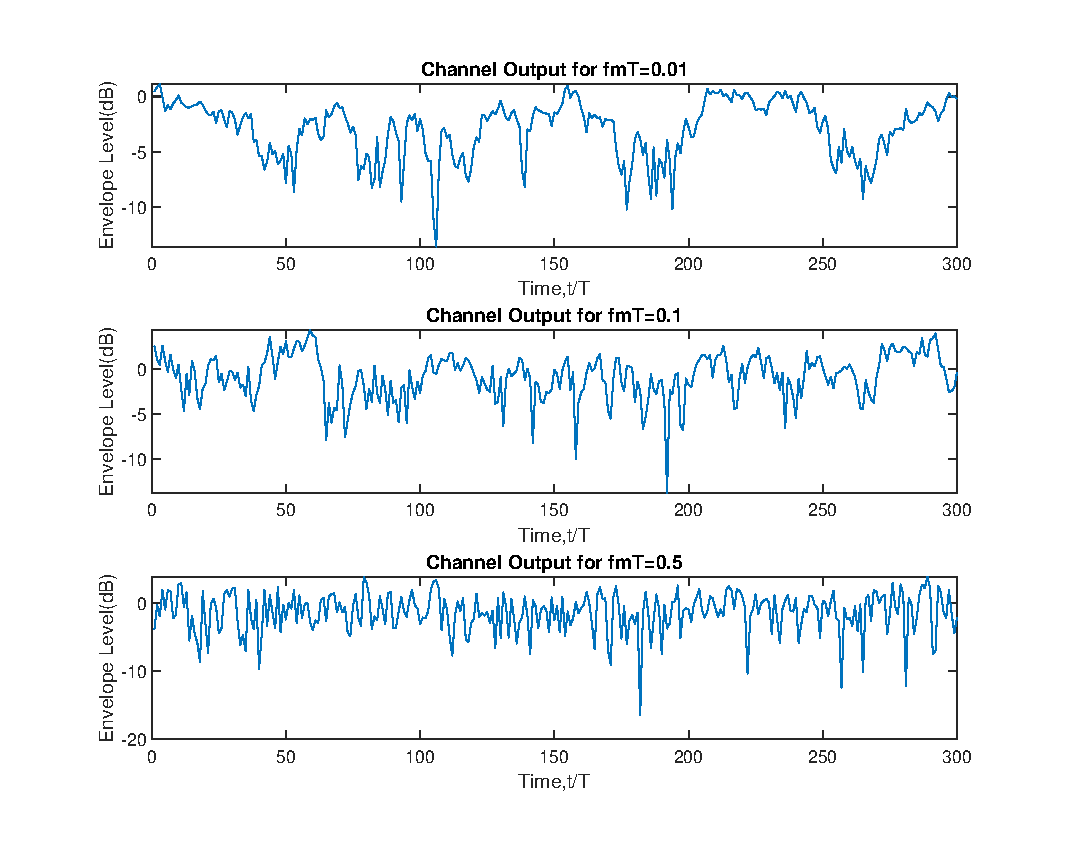
\includegraphics[scale = 0.7]{fg_envelop.eps}
\end{figure}
\begin{figure}[H]
    \centering
    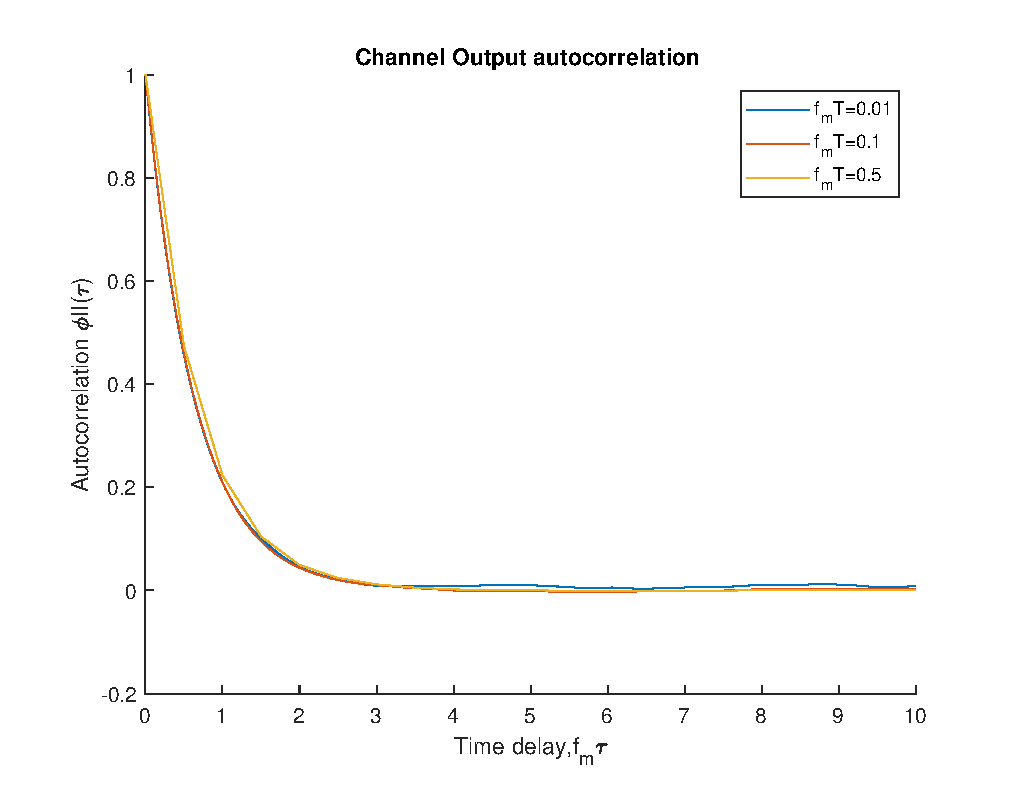
\includegraphics[scale = 0.7]{fg_auto.eps}
\end{figure}